\section{Software architecture and design}
\label{chapter2}

\paragraph
{}
	%If the acc is turned on, a 5ms task on Node 2 periodically requests distance readings from Node 1. Out of the readings it derives the new speed of the car. In alarm situations, e.g. failed readings, an object gets too close, no bt communication available, ... the acc turns off and alarms the driver to take over.
When the ACC is activated, Node 2 executes a periodic task every 5 ms to request distance measurements from Node 1. Based on these readings, it calculates the updated speed of the virtual car. In case of an alarm situation - such as invalid or missing sensor data, an object detected at critical distance, or a loss of Bluetooth communication - the ACC is automatically deactivated and the driver is alerted to take control.

\subsection{Software modules}

\begin{itemize}
	\item bt\_connection on Node 1 and Node 2
	\item acc\_control on Node 2
	\item proximity\_reader on Node 1
	\item display\_control on Node 2
	\item fault\_injection\_agent
\end{itemize}


\subsubsection{Safety related modules}
	% \begin{enumerate}
	% 	\item Modul x: \\
	% 		Description:\\
	% 		Functions:\\
	% 		Data:\\
	% 		Requirements see: \ref{req.1.1}, .... \\
	% \end{enumerate}


\subsubsection{Security related modules}

\subsubsection{Modules with no influence on Safety and Security}

\subsection{Libraries}

Description of used function with parameters.


\subsection{Interrupts}

Definition of priorities.

\subsection{Pinout}

In this subsection, the pinouts are presented separately for Node 1 and Node 2. Since both Nodes are based on a Raspberry Pi, the following diagram \ref{fig:raspi} shows the general pinout configuration of the Raspberry Pi.

\begin{figure}[h]
	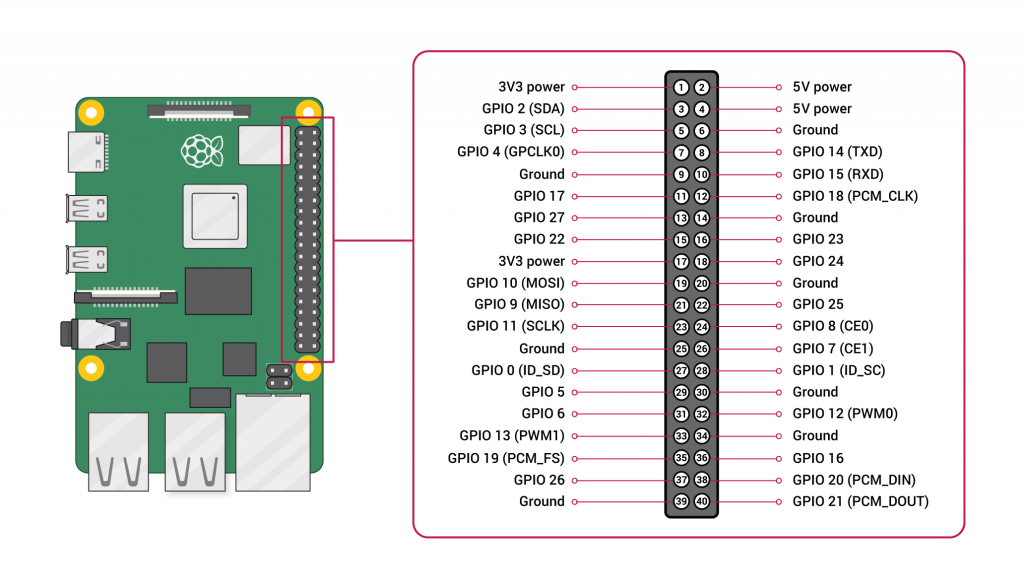
\includegraphics[height=50mm]{acc/doc/design/images/GPIO-Pinout-Diagram-2.png}
	\centering
	\caption{Raspberry Pi pinout configuration from \href{https://prilchen.de/raspberry-pis-gpio-ein-tor-zu-unzaehligen-projekten/} {prilchen.de}}
	\label{fig:raspi}
\end{figure}

\subsubsection{Node 1}

For Node 1, the ultrasonic sensor (HC-SR04) is connected to the Raspberry Pi. The VCC pin of the sensor is connected to the 5V power pin, while GND is connected to ground. The TRIG pin is wired to GPIO 23, and the ECHO pin is connected to GPIO 24 through a voltage divider using two resistors ($R_1 = 330\,\Omega$ and $R_2 = 470\,\Omega$) to safely reduce the signal from 5V to 3.3V. This can be viewed in Figure \ref{fig:node1-pinout}


\begin{figure}[h]
	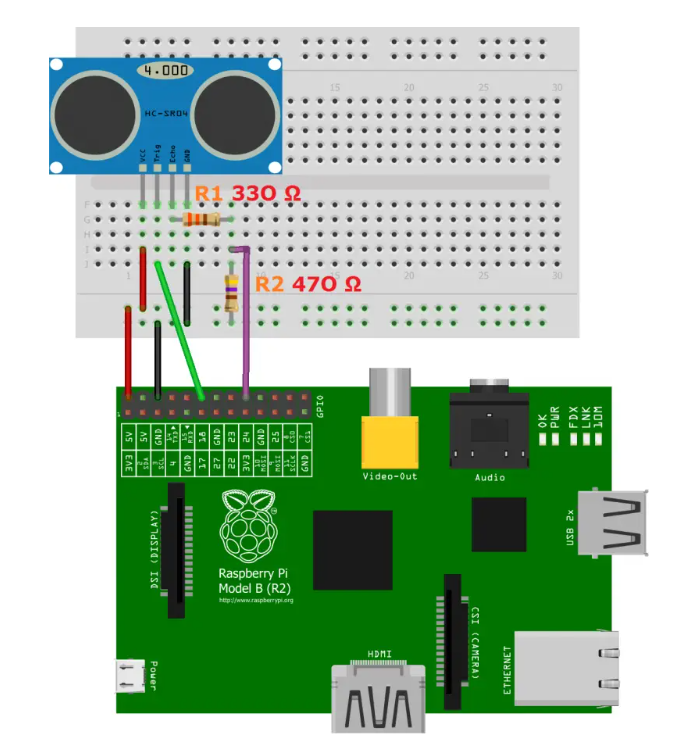
\includegraphics[height=50mm]{acc/doc/design/images/pinout_node1.png}
	\centering
	\caption{Pinout Node 1}
	\label{fig:node1-pinout}
\end{figure}

\subsubsection{Node 2}

For Node 2, the Raspberry Pi 4 is connected to the Raspberry Pi 7-inch Touch Display.  
The flat DSI ribbon cable is used to transmit the video signal and touch interface, while the four jumper wires provide power and enable I²C communication between the Raspberry Pi and the display controller. The wiring is as follows:

\begin{itemize}
    \item The \textbf{5V pin} of the display (marked ``5V'') is connected to the \textbf{5V power pin} of the Raspberry Pi (pin~4 on the GPIO header) \emph{(red cable)}.
    \item The \textbf{GND pin} of the display (marked ``GND'') is connected to the \textbf{ground pin} of the Raspberry Pi (pin~6 on the GPIO header) \emph{(black cable)}.
    \item The \textbf{SCL pin} of the display is connected to the \textbf{SCL pin} of the Raspberry Pi (pin~5 / GPIO~3) \emph{(yellow cable)}.
    \item The \textbf{SDA pin} of the display is connected to the \textbf{SDA pin} of the Raspberry Pi (pin~3 / GPIO~2) \emph{(green cable)}.
\end{itemize}

The wiring can be seen in Figure \ref{fig:node2-raspy} and \ref{fig:node2-display}.

\begin{figure}[h]
	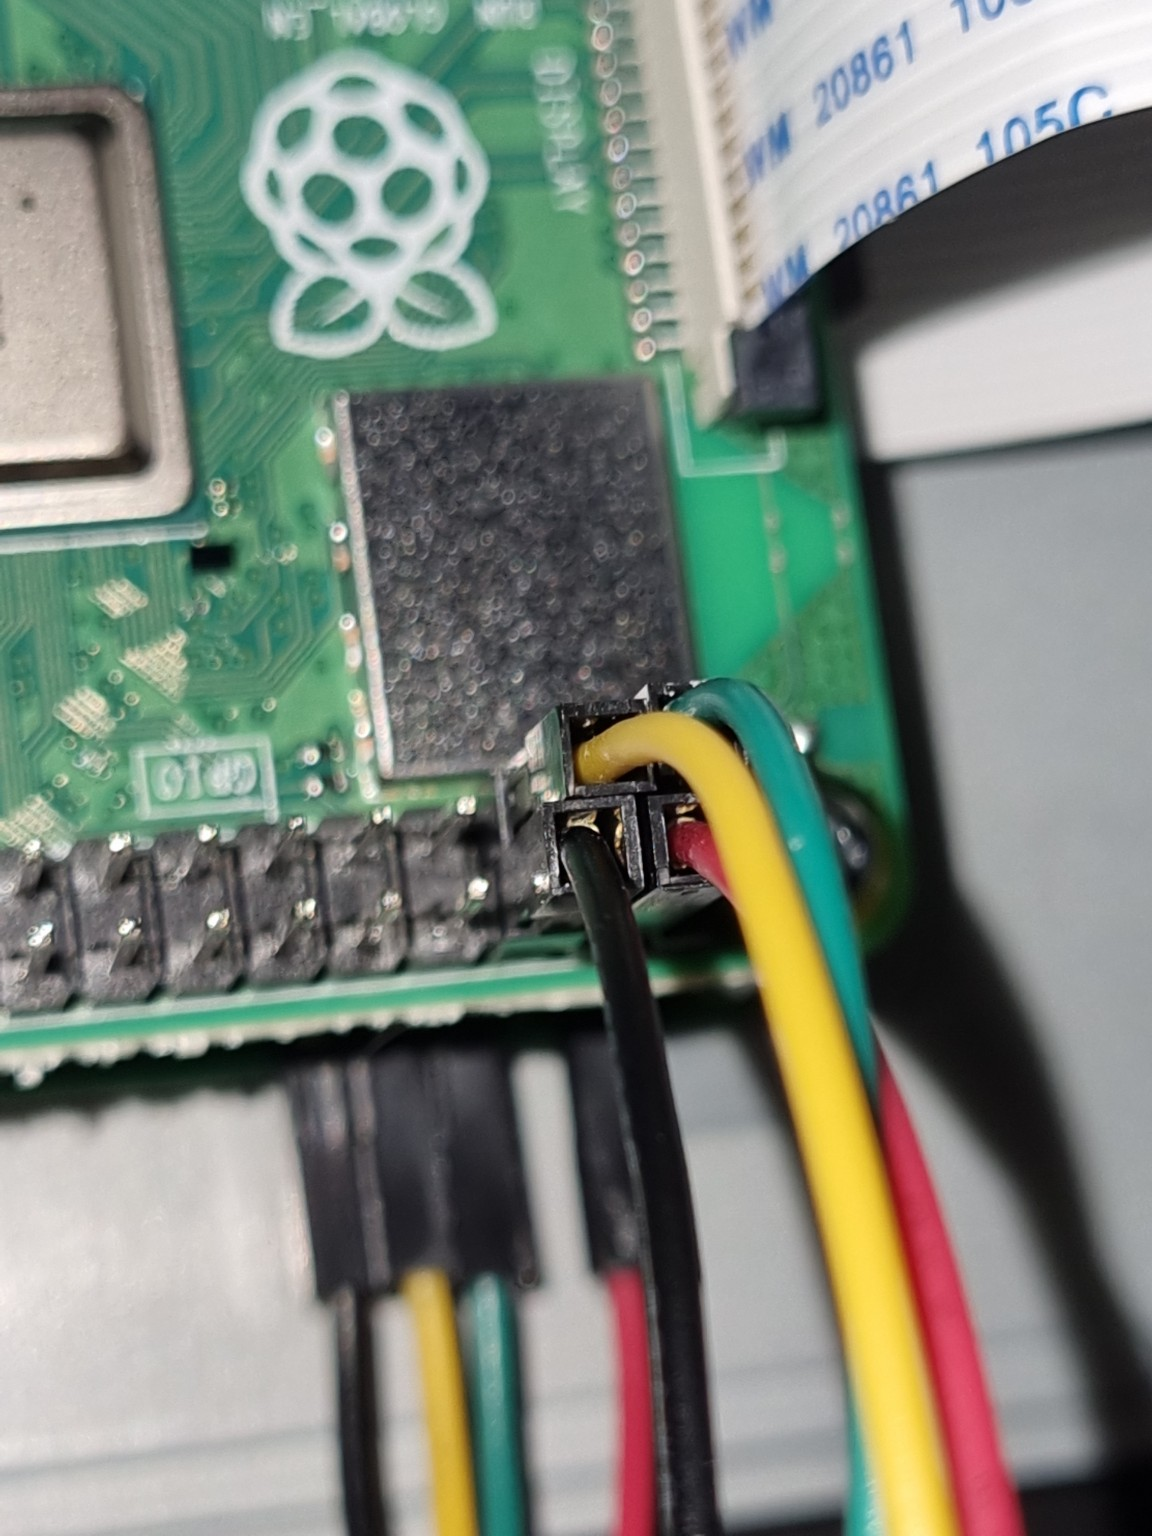
\includegraphics[height=100mm]{acc/doc/design/images/node2-raspy.jpg}
	\centering
	\caption{Pinout Node 2 Raspberry Pi}
	\label{fig:node2-raspy}
\end{figure}

\begin{figure}[h]
	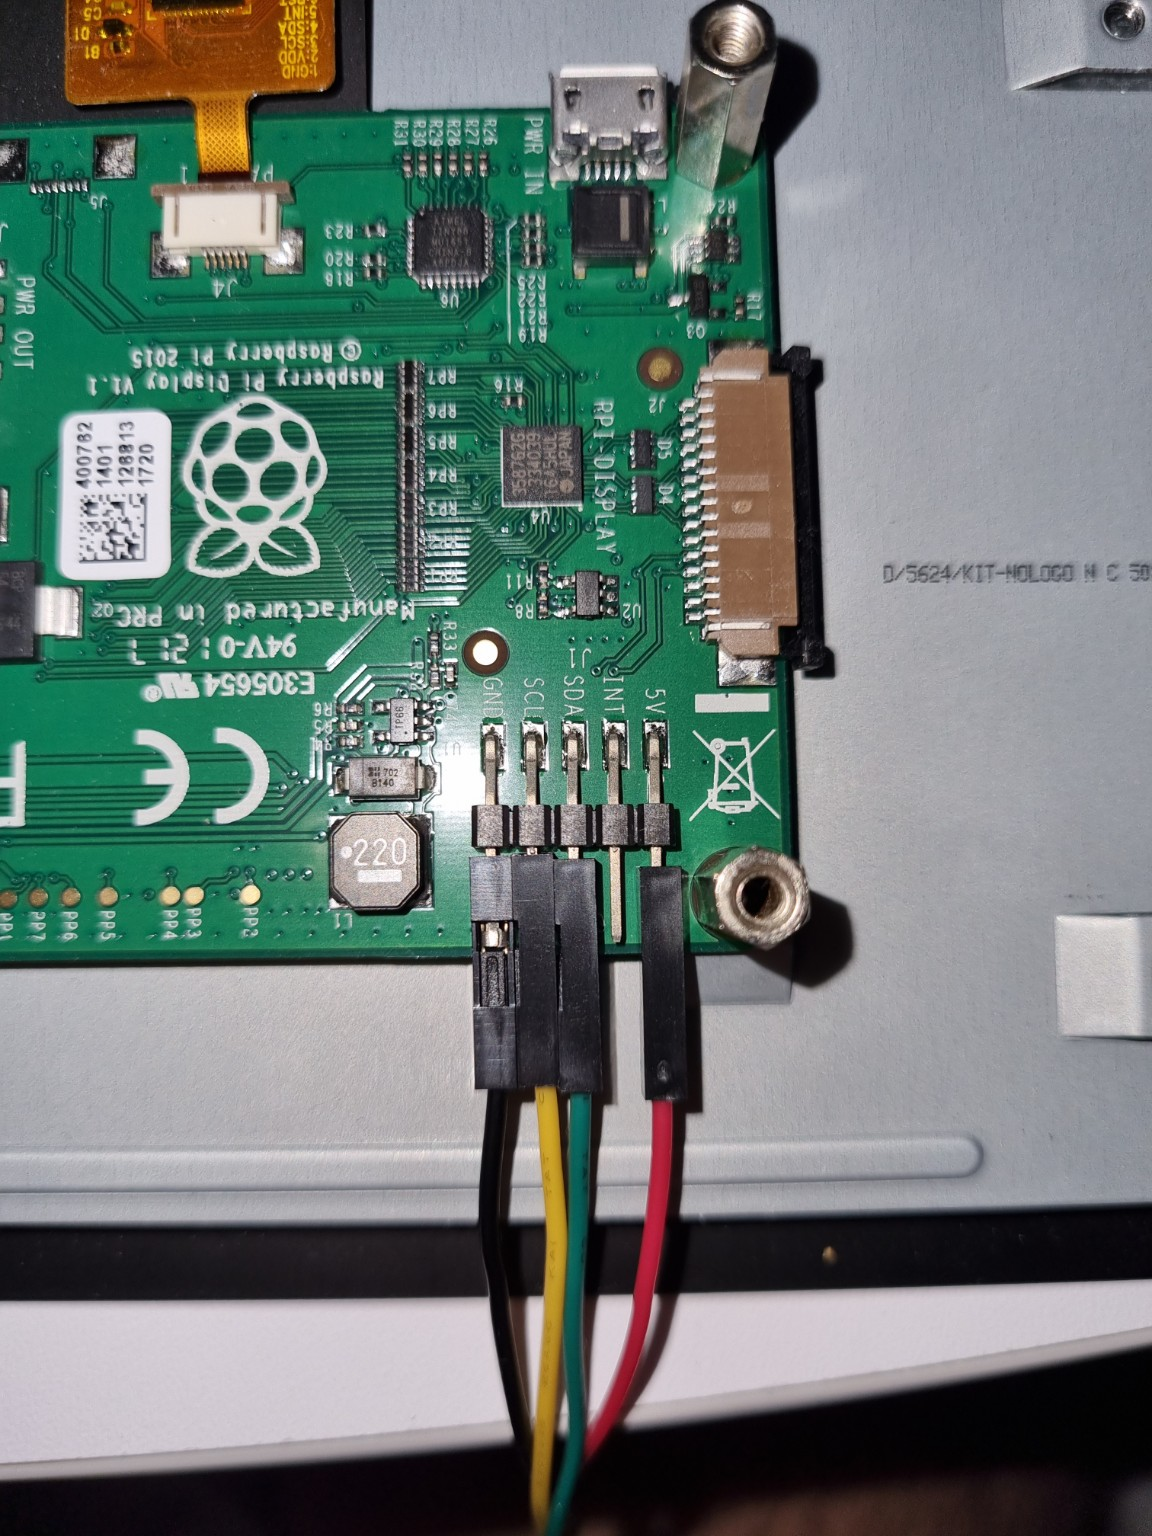
\includegraphics[height=100mm]{acc/doc/design/images/node2-display.jpg}
	\centering
	\caption{Pinout Node 2 Display}
	\label{fig:node2-display}
\end{figure}

\clearpage
\subsection{GUI}

Figure \ref{fig:gui} shows the dashboard GUI, containing the controls for accelerating and decelerating the vehicle, and for activating adaptive cruise control. It also contains elements showing the vehicles current speed, the distance to the nearest object in front of the car, and the status of the ACC system.

\begin{figure}[h]
	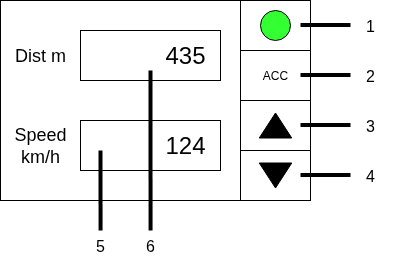
\includegraphics[height=50mm]{images/GUI.png}
	\centering
	\caption{Dashboard GUI}
	\label{fig:gui}
\end{figure}

\begin{enumerate}
  \item ACC Status LED: Shows the status of the ACC system, green if it is in an operational state, red, if ACC  is in a failed state.
  \item ACC Button: Push Button to activate ACC. Can only be pushed if ACC is in operational state.
  \item Accelerate Button: Increases the vehicle speed by 5 km/h (up to 200 km/h), deactivates ACC, if it was active.
  \item Decelerate Button: Decreases the vehicle speed by 5 km/h (down to 0 km/h), deactivates ACC, if it was active.
  \item Speed Display: Shows current vehicle speed
  \item Distance Display: Shows distance of the nearest object in front of the vehicle, does not display anything if ACC is in failed state.
\end{enumerate}

\subsection{Communication}

\paragraph{} Immediately after the communication is set up, Node 1 and Node 2 exchange 32 byte random numbers. These two numbers and a 32 byte pre-shared key are concatenated and put into a key derivation function returning a 256 bit AES session key used for HMAC generation. The message layout for these messages is shown in the first message in Figure \ref{fig:msg}.

\paragraph{}The messages which Node 1 and Node 2 are exchanging contain two fields:
\begin{itemize}
	\item MessageType: 1 byte, set to zero
	\item Random: 32 bytes, a random number generated by the sender node
\end{itemize}

FIXME: After key establishment, we should use a challenge-response round, so each participant proves to the other it owns the PSK. If that does not work on both sides, the connection should be dropped.

\paragraph{} After the common session key is established, the application uses a client server communication pattern, Node 1 acting as server and Node 2 acting as client. Node 2 periodically sends request messages to Node 1 which sends response messages. The message layout looks like depicted in the second and third messages in Figure \ref{fig:msg}. All multi byte fields are encoded as big-endian/in network byte order, i.e. the first byte of a field contains the MSB.

\paragraph{} All messages have the following layout:
\begin{itemize}
	\item MessageType: 1 byte, indicates the content of the Payload field
	\item Counter: 4 bytes, zero based 32 bit unsigned integer
	\item Payload: Holds the transmitted information
	\item HMAC: SHA-256 based HMAC, protecting all fields before the HMAC
\end{itemize}

\paragraph{} The request message, sent from Node 2 to Node 1, holds the \emph{Cmd} field, conveying the particular request to Node 2. Currently, only \emph{0x01} is supported, which requests the current distance reading from Node2.

\paragraph{} The response message, sent from Node 1 to Node 2, holds the \emph{Distance} field, conveying the most recent distance readings from Node1. In the error free case, that field holds values in the range of [0..400] indicating the measured distance to the next object in [m]. A value of \emph{0} indicates a measured distance below one meter, while a value of \emph{400} indicates a distance of 400 meters or a greater distance. A value of \emph{0xffff} indicates that both sensors yielded inconsistent readings (FIXME: Define what inconsistent means in our system), and the value of \emph{0xfffe} indicates that Node 1 detected a failure of one or both procimity sensors.


\begin{figure}[h]
	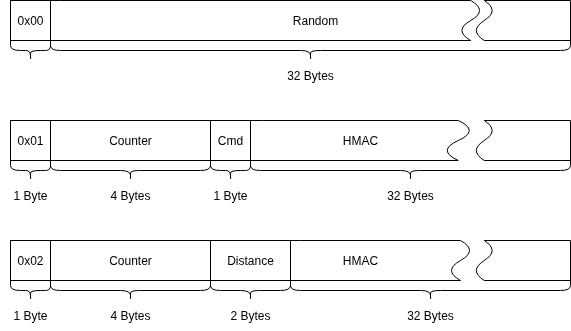
\includegraphics[height=50mm]{images/MessageLayout.png}
	\centering
	\caption{Layout of Messages}
	\label{fig:msg}
\end{figure}
